\documentclass[]{article}
\usepackage{lmodern}
\usepackage{amssymb,amsmath}
\usepackage{ifxetex,ifluatex}
\usepackage{fixltx2e} % provides \textsubscript
\ifnum 0\ifxetex 1\fi\ifluatex 1\fi=0 % if pdftex
  \usepackage[T1]{fontenc}
  \usepackage[utf8]{inputenc}
\else % if luatex or xelatex
  \ifxetex
    \usepackage{mathspec}
  \else
    \usepackage{fontspec}
  \fi
  \defaultfontfeatures{Ligatures=TeX,Scale=MatchLowercase}
\fi
% use upquote if available, for straight quotes in verbatim environments
\IfFileExists{upquote.sty}{\usepackage{upquote}}{}
% use microtype if available
\IfFileExists{microtype.sty}{%
\usepackage{microtype}
\UseMicrotypeSet[protrusion]{basicmath} % disable protrusion for tt fonts
}{}
\usepackage[margin=1in]{geometry}
\usepackage{hyperref}
\PassOptionsToPackage{usenames,dvipsnames}{color} % color is loaded by hyperref
\hypersetup{unicode=true,
            pdftitle={Additonal ASMA time Dublin (EIDW)},
            pdfauthor={Performance Review Unit, EUROCONTROL},
            colorlinks=true,
            linkcolor=Maroon,
            citecolor=Blue,
            urlcolor=blue,
            breaklinks=true}
\urlstyle{same}  % don't use monospace font for urls
\usepackage{longtable,booktabs}
\usepackage{graphicx,grffile}
\makeatletter
\def\maxwidth{\ifdim\Gin@nat@width>\linewidth\linewidth\else\Gin@nat@width\fi}
\def\maxheight{\ifdim\Gin@nat@height>\textheight\textheight\else\Gin@nat@height\fi}
\makeatother
% Scale images if necessary, so that they will not overflow the page
% margins by default, and it is still possible to overwrite the defaults
% using explicit options in \includegraphics[width, height, ...]{}
\setkeys{Gin}{width=\maxwidth,height=\maxheight,keepaspectratio}
\IfFileExists{parskip.sty}{%
\usepackage{parskip}
}{% else
\setlength{\parindent}{0pt}
\setlength{\parskip}{6pt plus 2pt minus 1pt}
}
\setlength{\emergencystretch}{3em}  % prevent overfull lines
\providecommand{\tightlist}{%
  \setlength{\itemsep}{0pt}\setlength{\parskip}{0pt}}
\setcounter{secnumdepth}{5}

%%% Use protect on footnotes to avoid problems with footnotes in titles
\let\rmarkdownfootnote\footnote%
\def\footnote{\protect\rmarkdownfootnote}

%%% Change title format to be more compact
\usepackage{titling}

% Create subtitle command for use in maketitle
\newcommand{\subtitle}[1]{
  \posttitle{
    \begin{center}\large#1\end{center}
    }
}

\setlength{\droptitle}{-2em}

  \title{Additonal ASMA time Dublin (EIDW)}
    \pretitle{\vspace{\droptitle}\centering\huge}
  \posttitle{\par}
  \subtitle{Approximation based on trajectory data}
  \author{Performance Review Unit, EUROCONTROL}
    \preauthor{\centering\large\emph}
  \postauthor{\par}
      \predate{\centering\large\emph}
  \postdate{\par}
    \date{20/02/2019}

\usepackage{flafter}
\usepackage{titlesec}
\newcommand{\sectionbreak}{\clearpage}
\makeatletter
\def\fps@figure{hbp}
\makeatother

\begin{document}
\maketitle

\section{Introduction}\label{introduction}

\subsection{General}\label{general}

This document provides results on an approximation for the additional
ASMA time for Dublin as calculated by the Performance Review Unit of
EUROCONTROL. More information on the methodology can be found on the
\href{http://http://ansperformance.eu/references/methodology/additional_asma_time_pi.html}{PRU
website}.

To calculate additional ASMA time using trajectory data only, the
methodology has been slightly adapted. The grouping of flights is done
by aircraft type group and ASMA sector, but not by runway since that
information is not available nor obtainable from the trajectory data.

\subsection{Acronyms and terminology}\label{acronyms-and-terminology}

\begin{longtable}[]{@{}ll@{}}
\toprule
\begin{minipage}[b]{0.09\columnwidth}\raggedright\strut
Term\strut
\end{minipage} & \begin{minipage}[b]{0.33\columnwidth}\raggedright\strut
Definition\strut
\end{minipage}\tabularnewline
\midrule
\endhead
\begin{minipage}[t]{0.09\columnwidth}\raggedright\strut
ASMA\strut
\end{minipage} & \begin{minipage}[t]{0.33\columnwidth}\raggedright\strut
Arrival Sequencing and Metering Area\strut
\end{minipage}\tabularnewline
\begin{minipage}[t]{0.09\columnwidth}\raggedright\strut
PRU\strut
\end{minipage} & \begin{minipage}[t]{0.33\columnwidth}\raggedright\strut
Performance Review Unit\strut
\end{minipage}\tabularnewline
\bottomrule
\end{longtable}

\newpage

\section{Results over time}\label{results-over-time}

The additional ASMA time for Dublin over time is shown in Figure
\ref{fig:ASMAtime}.

\begin{figure}

{\centering 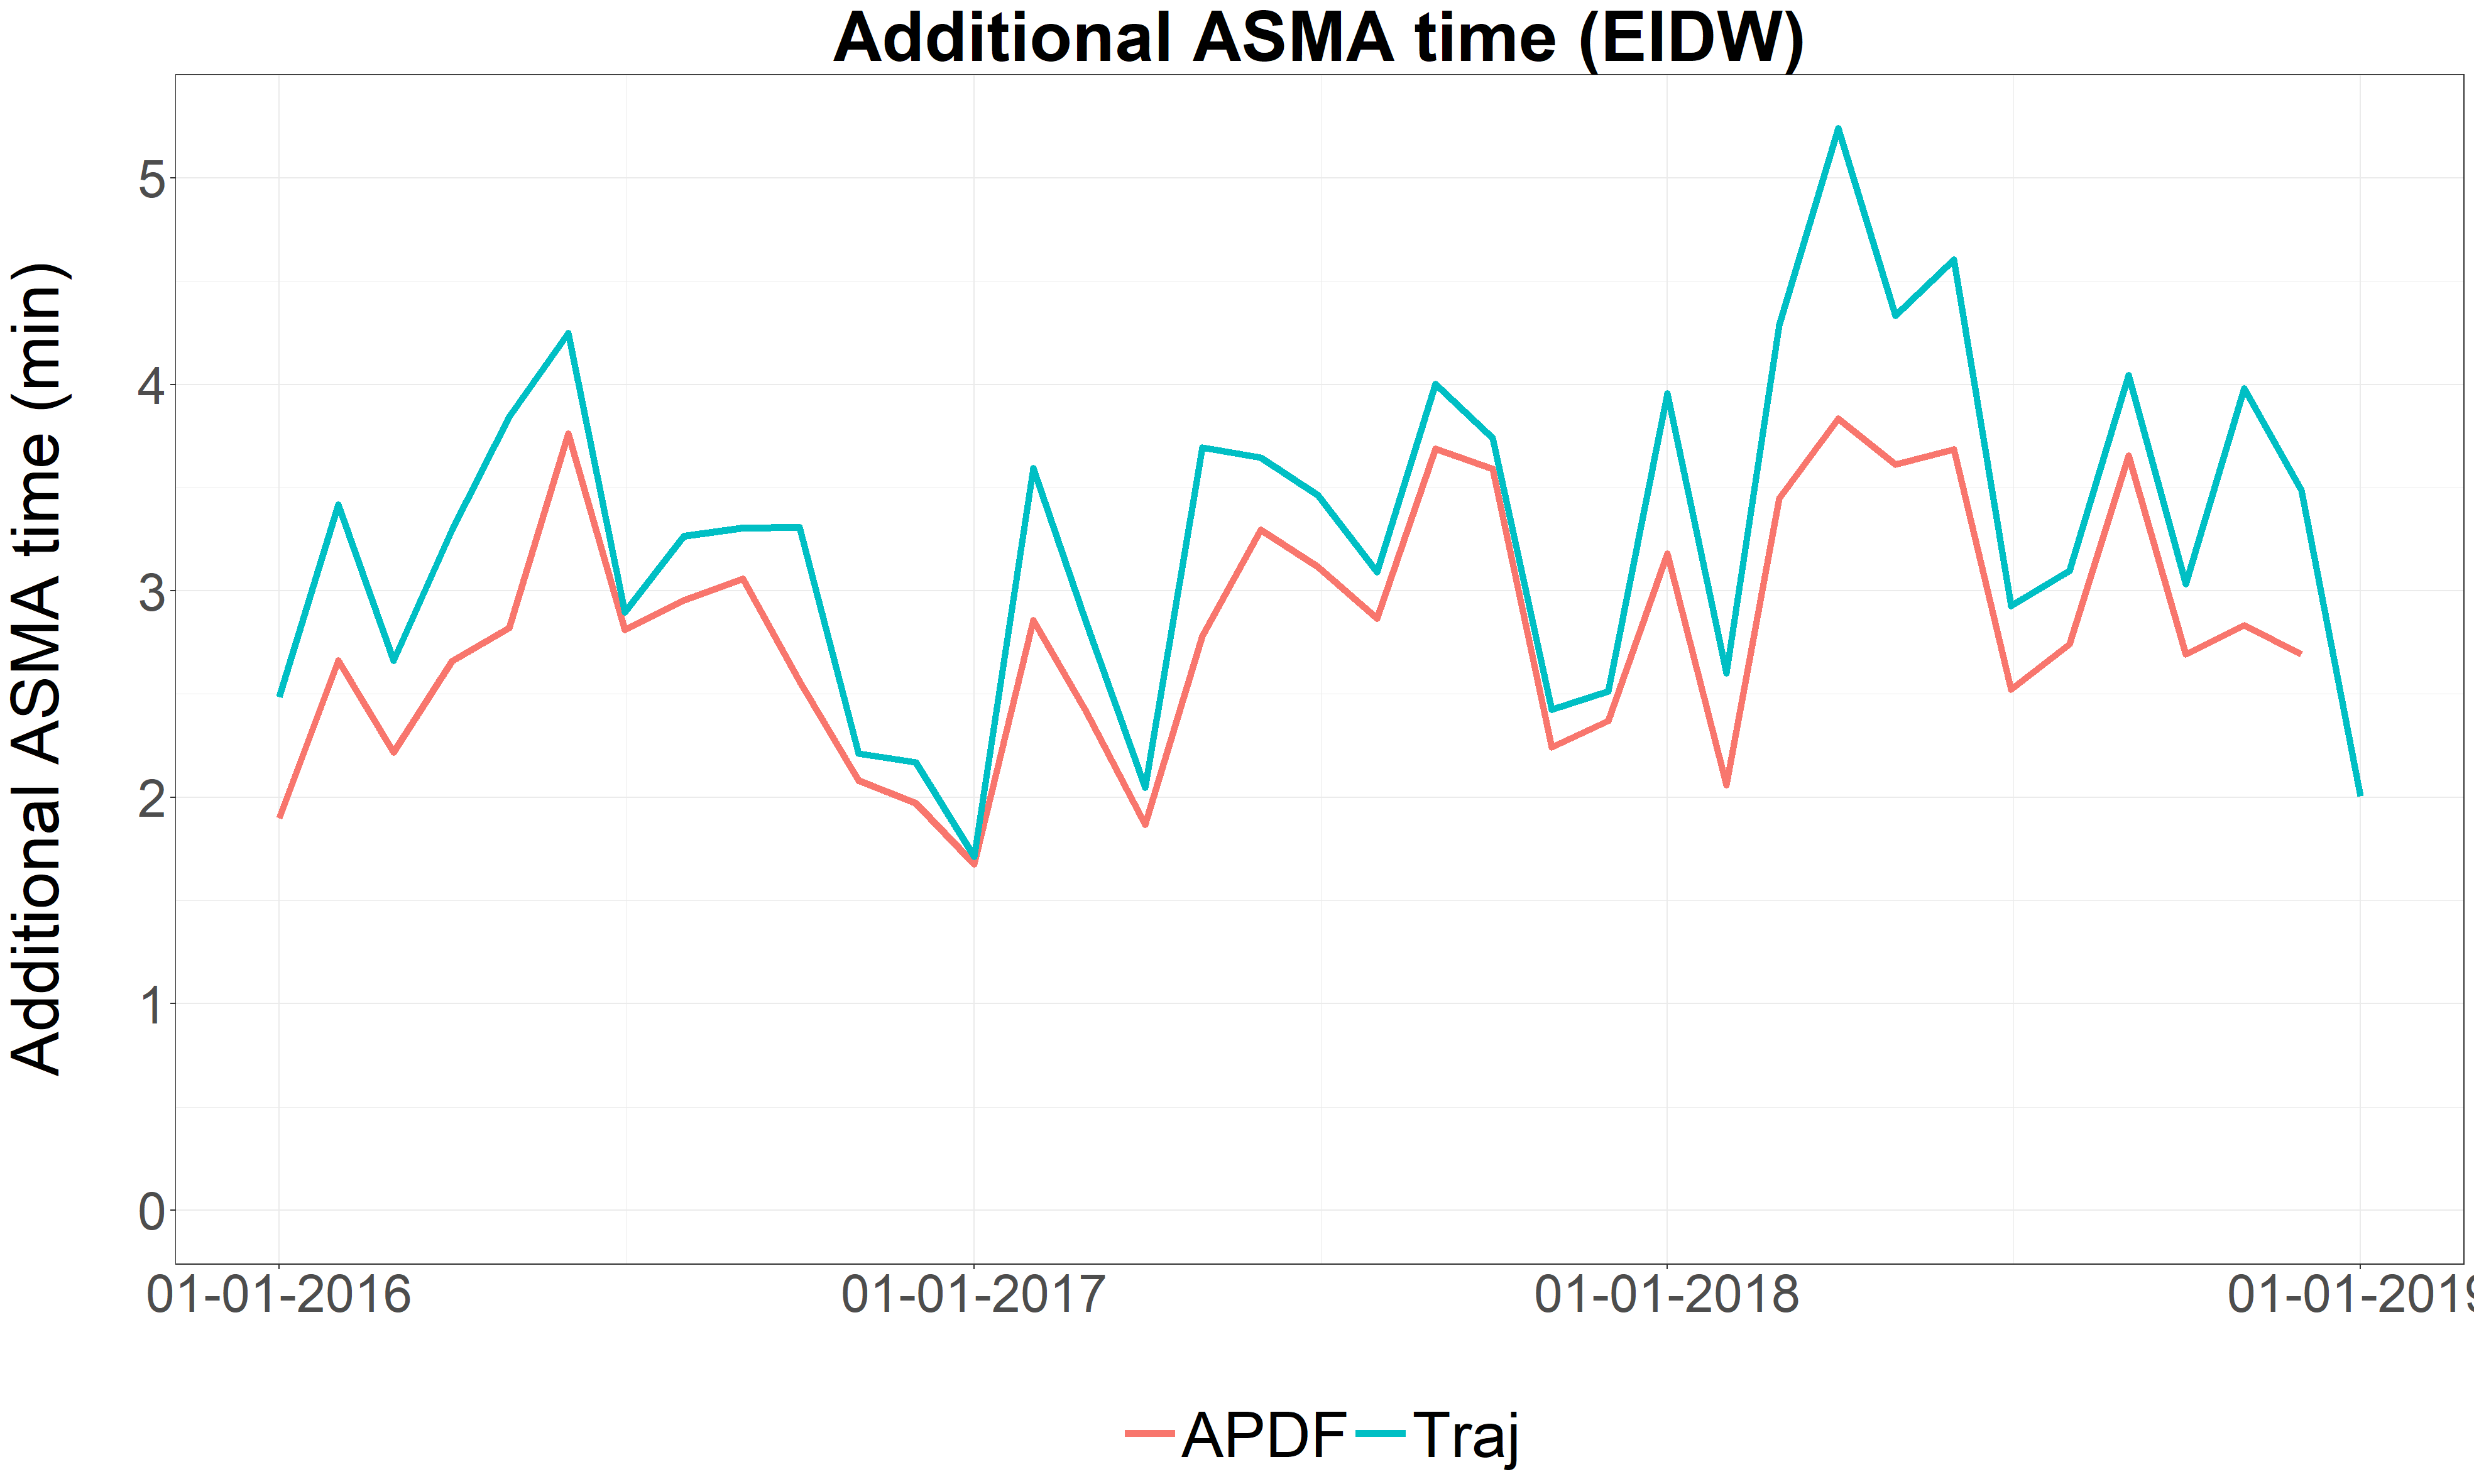
\includegraphics[width=\textwidth]{//hhbruna30/dgof-pru$/Project/Vertical_flight_efficiency/2015/ASMA_approx/Figures/Additional_ASMA_EIDW} 

}

\caption{Additional ASMA time}\label{fig:ASMAtime}
\end{figure}


\end{document}
